\section{计算目标与精度要求}
\label{sec:budget-targets}

比较方法之前，先要说清楚算什么、算到什么程度算完。待算的量是固定的数：积分$I=\mathbb{E}_{\pi}[f]$，或者含参期望$J(\bm{\theta})$在某一点的梯度$\nabla J(\bm{\theta})\in\mathbb{R}^{d}$。随机的是计算过程，估计$\hat{I}_n$随所用随机数而变。“精度”因此是对$\hat{I}_n-I$这个随机误差的要求，而同一个误差可以用几种不同的方式来约束。不同的约束会要求很不一样的样本数，有的在目标接近零时还会失去意义。

\paragraph{三种误差口径}
最直接的要求是误差的绝对值$\lvert\hat{I}_n-I\rvert$不超过给定的$\varepsilon$。但$\hat{I}_n$是随机的，任何有限样本都可能偶然偏得很远，所以“误差不超过$\varepsilon$”只能以平均或概率的方式表达。第一种是要求\term{均方误差}（mean squared error）不超过$\varepsilon^{2}$。按第~\ref{chap:monte-carlo-integration-error}章的分解，在$\hat{I}_n$二阶矩有限时
\begin{equation}
  \mathbb{E}\bigl[(\hat{I}_n-I)^{2}\bigr]=\bigl(\mathbb{E}[\hat{I}_n]-I\bigr)^{2}+\operatorname{Var}(\hat{I}_n),
  \label{eq:budget-mse}
\end{equation}
右边第一项是偏差的平方，第二项是随机波动。均方误差把两者放在同一个单位下相加，便于在它们之间权衡。

第二种是指定概率下的误差：给定容差$\varepsilon>0$和允许的失败概率$\delta\in(0,1)$，要求
\begin{equation}
  \mathbb{P}\bigl(\lvert\hat{I}_n-I\rvert>\varepsilon\bigr)\le\delta .
  \label{eq:budget-eps-delta}
\end{equation}
它直接回答“这次计算有多大把握落在容差以内”。两种口径之间有一个总成立的桥：对误差平方用Markov不等式，
\[
  \mathbb{P}\bigl(\lvert\hat{I}_n-I\rvert>\varepsilon\bigr)\le\frac{\mathbb{E}\bigl[(\hat{I}_n-I)^{2}\bigr]}{\varepsilon^{2}} .
\]
所以只要均方误差不超过$\delta\varepsilon^{2}$，式~\eqref{eq:budget-eps-delta}就成立。这一步不需要任何分布假设，代价是保守。

对独立同分布、方差为$\sigma^{2}$的无偏样本平均，$\operatorname{Var}(\hat{I}_n)=\sigma^{2}/n$，上面的充分条件给出样本数
\begin{equation}
  n_{\mathrm{Cheb}}=\frac{\sigma^{2}}{\delta\varepsilon^{2}} .
  \label{eq:budget-n-cheb}
\end{equation}
若改用中心极限定理的正态近似，记$z_{1-\delta/2}$为标准正态的$1-\delta/2$分位数，需要的样本数约为
\begin{equation}
  n_{\mathrm{N}}\approx\frac{z_{1-\delta/2}^{2}\,\sigma^{2}}{\varepsilon^{2}} .
  \label{eq:budget-n-normal}
\end{equation}
后者只是渐近近似，覆盖保证不是有限样本下精确的；前者是有限样本下成立的上界。两者的差别完全来自对$\delta$的依赖：Chebyshev界按$1/\delta$增长，正态近似中的$z_{1-\delta/2}^{2}$只按$\ln(1/\delta)$的量级增长。

以$\mathrm{e}^{u}$在$[0,1]$上的积分$I=\mathrm{e}-1$为例，直接平均$\mathrm{e}^{U}$的单样本方差是
\[
  \sigma^{2}=\frac{\mathrm{e}^{2}-1}{2}-(\mathrm{e}-1)^{2}\approx0.2420 .
\]
取$\varepsilon=0.01$、$\delta=0.05$，由式~\eqref{eq:budget-n-cheb}与式~\eqref{eq:budget-n-normal}，
\[
  n_{\mathrm{Cheb}}=\frac{0.2420}{0.05\times10^{-4}}\approx48\,400,\qquad n_{\mathrm{N}}\approx\frac{1.96^{2}\times0.2420}{10^{-4}}\approx9\,300 .
\]
两者相差约$5.2$倍。图~\ref{fig:budget-n-requirement}(a)画出$\delta$变化时这两个样本数：$\delta$越小，Chebyshev界与正态近似的距离越大。选择哪一个，要看报告需要有限样本的保证，还是可以接受渐近近似。

\begin{BookInlineFigure}
  \centering
  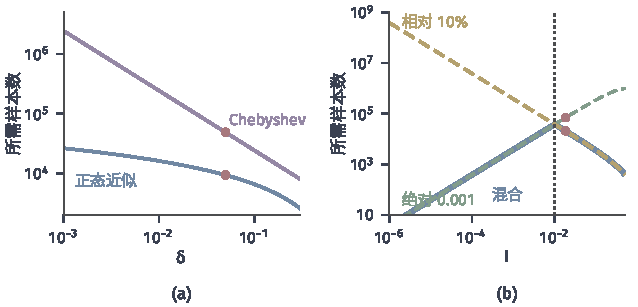
\includegraphics[width=108mm]{figures/07-probability/08-sampling-and-integration/matplotlib/budget-n-requirement/figure.pdf}
  \caption{误差口径决定所需样本数。(a)~积分$\mathrm{e}-1$、容差$\varepsilon=0.01$：紫线为Chebyshev界式~\eqref{eq:budget-n-cheb}，蓝线为正态近似式~\eqref{eq:budget-n-normal}，红点为$\delta=0.05$。(b)~尾概率$I$的直接平均在$95\%$正态近似下所需的样本数：绿色虚线为绝对容差$0.001$，黄色虚线为相对容差$10\%$，蓝色粗线为二者取较宽者的混合容差；竖直点线$I=0.01$是两种容差相等处，红点对应$I=\mathrm{e}^{-4}$。}
  \label{fig:budget-n-requirement}
\end{BookInlineFigure}

梯度的目标是向量$\nabla J(\bm{\theta})\in\mathbb{R}^{d}$，误差用欧氏范数衡量。设估计$\hat{\bm{g}}$的均值为$\bm{m}$，协方差矩阵为$\bm{\Sigma}_{\hat{g}}$，逐分量应用式~\eqref{eq:budget-mse}再相加，得到
\begin{equation}
  \mathbb{E}\bigl[\lVert\hat{\bm{g}}-\nabla J\rVert_2^{2}\bigr]=\lVert\bm{m}-\nabla J\rVert_2^{2}+\operatorname{tr}\bm{\Sigma}_{\hat{g}} .
  \label{eq:budget-vector-mse}
\end{equation}
波动部分是协方差矩阵的迹，即各分量方差之和。若只关心某个方向$\bm{v}$上的变化率，相应的误差只涉及$\bm{v}^{\top}\bm{\Sigma}_{\hat{g}}\bm{v}$，比全向量的要求宽松得多。第~\ref{sec:budget-gradient-choice}节会看到，按迹比较时各种梯度估计的优劣可能与按单个分量比较时不同。

\paragraph{相对误差与接近零的目标}
当待算量很小时，绝对容差$0.001$可能比答案本身还大，于是人们常改用\term{相对误差}（relative error）$\lvert\hat{I}_n-I\rvert/\lvert I\rvert$。对尾概率，相对要求才有意义：$I=\mathrm{e}^{-4}\approx0.0183$时，报告$0.0183\pm0.001$与报告$0.0183\pm0.0002$说明的事情差别不大，但报告$0.0183\pm0.0183$就没有说明任何事。问题出在$I$趋于零时。直接平均示性函数的单样本方差是$I(1-I)$，相对容差$\varepsilon_{\mathrm{rel}}$在正态近似下要求
\[
  n\approx\frac{z^{2}I(1-I)}{(\varepsilon_{\mathrm{rel}}I)^{2}}=\frac{z^{2}(1-I)}{\varepsilon_{\mathrm{rel}}^{2}\,I},
\]
其中$z=1.96$。它随$I\to0$按$1/I$增长；$I=0$时这个要求无法满足，因为任何非零的估计都有无穷大的相对误差。

目标恰为零或可能为零的情形很常见：一个奇函数在对称分布下的期望，参数取到最优点时的梯度，两种方案期望之差在二者一样好时的取值。这时只用相对误差会使计算无限进行下去。实用的写法是给一个\term{混合容差}（mixed tolerance）：
\begin{equation}
  \lvert\hat{I}_n-I\rvert\le\max\bigl\{\varepsilon_{\mathrm{abs}},\ \varepsilon_{\mathrm{rel}}\lvert I\rvert\bigr\} .
  \label{eq:budget-mixed-tolerance}
\end{equation}
目标较大时相对项起作用，目标接近零时绝对项兜底。对梯度，把式中的绝对值换成欧氏范数即可；在参数接近最优点时梯度本身趋于零，这时只有绝对项能给出可以达到的要求。$\varepsilon_{\mathrm{abs}}$不是随意的：它表示“比这更小的差别对使用者已无意义”的尺度，应由任务本身给出。

用尾概率走一遍。$I=\mathrm{e}^{-4}$时单样本方差$I(1-I)\approx0.01798$。绝对容差$0.001$与相对容差$10\%$在正态近似下分别要求
\[
  n_{\mathrm{abs}}\approx\frac{1.96^{2}\times0.01798}{10^{-6}}\approx69\,100,\qquad n_{\mathrm{rel}}\approx\frac{1.96^{2}\times0.9817}{0.01\times0.01832}\approx20\,600 .
\]
混合容差取二者中较宽的$\max\{0.001,0.00183\}=0.00183$，所需样本数就是$20\,600$。图~\ref{fig:budget-n-requirement}(b)把这三条曲线画成$I$的函数：相对容差的曲线在$I\to0$时向上发散，绝对容差的曲线向下，混合容差取二者的较小者，在两种容差相等的$I=0.01$处转折。

还要注意：混合容差里的$\lvert I\rvert$本身未知，实际判断只能用估计值代替。这个代替在估计值远离零时无害，在估计值接近零时会把相对项估得过小或过大，第~\ref{sec:budget-stopping}节讨论依据数据决定何时停止时还会回到这一点。

\paragraph{固定预算与固定精度}
同一个误差要求可以从两个方向提出。一是预算$C$给定，在所有可行方案中使误差最小；二是误差要求给定，使达到它的成本最小。用均方误差写，二者分别是
\begin{equation}
  \min_{\text{方案}}\ \mathrm{MSE}\quad\text{使}\ \text{成本}\le C,
  \qquad
  \min_{\text{方案}}\ \text{成本}\quad\text{使}\ \mathrm{MSE}\le\varepsilon^{2}.
  \label{eq:budget-two-problems}
\end{equation}
对无偏的独立样本平均，两个问题等价。设每个样本的成本为$c$、方差为$\sigma^{2}$，预算$C$可买$n=C/c$个样本，于是
\begin{equation}
  \mathrm{MSE}\cdot C=\frac{\sigma^{2}}{n}\cdot nc=\sigma^{2}c .
  \label{eq:budget-mse-cost-product}
\end{equation}
乘积$\sigma^{2}c$与预算无关：给定预算时误差是$\sigma^{2}c/C$，给定误差时成本是$\sigma^{2}c/\varepsilon^{2}$，哪个方案的$\sigma^{2}c$小，它在两种提法下都更好。第~\ref{sec:budget-costs}节会把$\sigma^{2}c$作为比较的基本量。

有偏差时情况不同。偏差不随样本数减小，它通常由方法的某个参数控制，例如数值离散的步长；而缩小偏差往往使每个有效样本更贵。这时固定预算与固定精度的答案都要在偏差和波动之间折中，而且固定精度的问题可能对某些参数根本无解：若偏差本身已经超过$\varepsilon$，增加样本只会把误差压到偏差为止。

下面用第~\ref{chap:monte-carlo-integration-error}章的近似链说明这种折中。目标是$\pi=\mathcal{N}(0,1)$，被积函数$f(x)=x^{2}$，$I=1$。用步长$h\in(0,1)$的链
\begin{equation}
  X^{(t+1)}=(1-h)X^{(t)}+\sqrt{2h}\,\varepsilon^{(t)},\qquad\varepsilon^{(t)}\sim\mathcal{N}(0,1)\ \text{独立},
  \label{eq:budget-ula-chain}
\end{equation}
每步成本记为$1$。这条链的不变分布不是目标：对平稳的方差$v$，由$v=(1-h)^{2}v+2h$解得$v=2/(2-h)$。于是平稳时的偏差
\[
  b(h)=v-1=\frac{h}{2-h}.
\]

再算波动。记$\rho=1-h$。平稳的高斯自回归链中，$X^{(0)}$与$X^{(k)}$是协方差为$v\rho^{k}$的联合高斯变量，由高斯四阶矩公式，
\[
  \operatorname{Cov}\bigl((X^{(0)})^{2},(X^{(k)})^{2}\bigr)=2\bigl(v\rho^{k}\bigr)^{2}=2v^{2}\rho^{2k}.
\]
代入第~\ref{chap:monte-carlo-integration-error}章的长期方差（$\gamma_{0}$加上各阶自协方差之和的两倍），对几何级数求和，得到
\[
  \sigma_{\mathrm{LR}}^{2}(h)=2v^{2}\Bigl(1+2\sum_{k\ge1}\rho^{2k}\Bigr)=\frac{2v^{2}(1+\rho^{2})}{1-\rho^{2}}=\frac{2v^{2}\bigl(1+(1-h)^{2}\bigr)}{h(2-h)} .
\]
从平稳状态启动、运行$B$步时，均方误差在$B$较大时为
\begin{equation}
  \mathrm{MSE}(h,B)\approx b(h)^{2}+\frac{\sigma_{\mathrm{LR}}^{2}(h)}{B} .
  \label{eq:budget-ula-mse}
\end{equation}
步长越小，偏差越小，但链的相关越强，波动越大。

对小$h$取主项，$b(h)\approx h/2$，$\sigma_{\mathrm{LR}}^{2}(h)\approx2/h$，于是
\[
  \mathrm{MSE}(h,B)\approx\frac{h^{2}}{4}+\frac{2}{hB}.
\]
对$h$求导并令其为零，$h/2-2/(h^{2}B)=0$，解得最优步长和最小均方误差
\begin{equation}
  h^{\ast}\approx\Bigl(\frac{4}{B}\Bigr)^{1/3},\qquad\mathrm{MSE}^{\ast}\approx\frac34\cdot4^{2/3}B^{-2/3}\approx1.89\,B^{-2/3}.
  \label{eq:budget-ula-opt}
\end{equation}
均方根误差按$B^{-1/3}$下降，比无偏样本平均的$B^{-1/2}$慢。原因是每增加预算，最优安排都要把一部分花在缩小步长上，而不是全部用于平均。

图~\ref{fig:budget-ula-tradeoff}(a)按式~\eqref{eq:budget-ula-mse}的精确表达式画出三种预算下的均方误差：左侧是波动主导，右侧贴近偏差平方$b(h)^{2}$，红点是最优步长。$B=10^{4}$时数值最优$h^{\ast}\approx0.071$，均方误差约$0.0043$，均方根误差约$0.065$；从$\mathcal{N}(0,1)$直接独立抽样时$\operatorname{Var}(X^{2})=2$，同样预算的均方根误差是$\sqrt{2/10^{4}}\approx0.014$。图~\ref{fig:budget-ula-tradeoff}(b)比较两种方法达到均方根误差$\varepsilon=0.01$所需的预算：精确采样需要$2/\varepsilon^{2}=2\times10^{4}$步，近似链即使每次都取最优步长也需要约$2.6\times10^{6}$步。

\begin{BookInlineFigure}
  \centering
  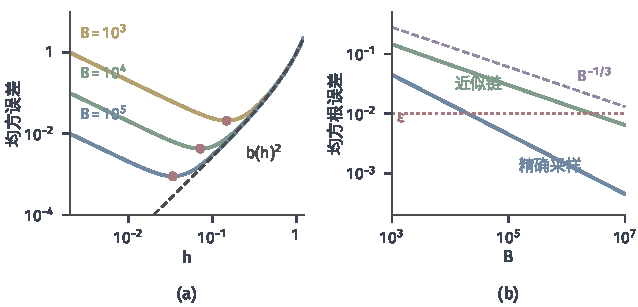
\includegraphics[width=108mm]{figures/07-probability/08-sampling-and-integration/matplotlib/budget-ula-tradeoff/figure.pdf}
  \caption{近似链~\eqref{eq:budget-ula-chain}在偏差与波动之间的折中，$f(x)=x^{2}$，目标$\mathcal{N}(0,1)$，从平稳状态启动。(a)~三种预算$B$下的均方误差随步长$h$变化，深灰虚线为偏差平方$b(h)^{2}$，红点为最优步长。(b)~均方根误差随预算变化：蓝线为独立精确抽样，绿线为每个预算下取最优步长的近似链，紫色虚线为$B^{-1/3}$参考斜率，红色点线为容差$\varepsilon=0.01$。}
  \label{fig:budget-ula-tradeoff}
\end{BookInlineFigure}

这个例子还说明，式~\eqref{eq:budget-two-problems}两种提法的结论都依赖偏差项是否存在。对无偏方法，只需比较$\sigma^{2}c$；对有偏方法，必须同时选择控制偏差的参数，固定精度的要求会把预算推到偏差允许的范围。式~\eqref{eq:budget-ula-mse}忽略了初值的影响，从非平稳状态启动时还要加上第~\ref{chap:monte-carlo-integration-error}章所说的初始偏差，它在这里按$1/(hB)$衰减，不改变$B^{-1/3}$的量级。
